\documentclass[oneside,a4paper,14pt]{extarticle}
\usepackage[a4paper,letterpaper,top=20mm,bottom=20mm,left=20mm,right=10mm]{geometry}
\usepackage[russian]{babel}
\usepackage{indentfirst}
\usepackage{graphicx}
\usepackage{caption}
\usepackage{titlesec}
\usepackage{verbatim, fancyvrb}

\titleformat{\section} {\normalsize\bfseries} {\thesection} {1em} {}
\titleformat{\subsection} {\normalsize\bfseries} {\thesubsection} {1em} {}
\titleformat{\subsubsection} {\normalsize\bfseries} {\thesubsection} {1em} {}
\renewcommand\baselinestretch{1.45}\normalsize
\setlength{\parindent}{1.25cm}

\begin{document}

\newpage
\thispagestyle{empty}
\begin{center}
	МИНИСТЕРСТВО НАУКИ И ВЫСШЕГО ОБРАЗОВАНИЯ РОССИЙСКОЙ ФЕДЕРАЦИИ ФЕДЕРАЛЬНОЕ ГОСУДАРСТВЕННОЕ БЮДЖЕТНОЕ ОБРАЗОВАТЕЛЬНОЕ УЧРЕЖДЕНИЕ ВЫСШЕГО ОБРАЗОВАНИЯ\\
	«ВЯТСКИЙ ГОСУДАРСТВЕННЫЙ УНИВЕРСИТЕТ»\\
	Институт математики и информационных систем\\
	Факультет автоматики и вычислительной техники\\
	Кафедра электронных вычислительных машин
\end{center}
\vspace{10mm}

\hfill
\begin{tabular}{l}
  \footnotesize Дата сдачи на проверку: \\
  \footnotesize <<\rule[-1mm]{5mm}{0.10mm}\/>>\rule[-1mm]{20mm}{0.10mm}\ 2024 г.\\
  \footnotesize Проверено: \\
  \footnotesize <<\rule[-1mm]{5mm}{0.10mm}\/>>\rule[-1mm]{20mm}{0.10mm}\ 2024 г. \\
\end{tabular}
\vfill

\begin{center}
    РЕАЛИЗАЦИЯ И РАБОТА С ДВУСВЯЗНЫМ СПИСКОМ\\
	Отчёт по лабораторной работе №3\\
	по дисциплине\\
	<<Программирование>>\\
\end{center}
\vspace{30mm}
\noindent
\begin{tabular}{ll}
	Разработал студент гр. ИВТб-1301-05-00 & \rule[-1mm]{30mm}{0.10mm}\,/Черкасов А. А./   \\
	                                       & \hspace{8mm}\footnotesize(подпись)            \\
	Заместитель кафедры ЭВМ                & \rule[-1mm]{30mm}{0.10mm}\,/Долженкова М. Л./ \\
	                                       & \hspace{8mm}\footnotesize(подпись)            \\
\end{tabular}

\noindent
  \begin{tabular}{lp{58mm}r}
    Работа защищена &  & <<\rule[-1mm]{5mm}{0.10mm}\/>>\rule[-1mm]{30mm}{0.10mm}\ 2024 г.
  \end{tabular}
  \vfill

\begin{center}
	Киров\\
	2024
\end{center}

\newpage\thispagestyle{plain}

\section*{Цель}

Цель работы: Изучить структуру данных "двусвязный список" и принципы работы с ним. Реализовать операции добавления, удаления и вывода элементов списка. Разработать программу с интерактивным вводом данных и поддержкой управления списком через команды.

\section*{Задание}
\begin{itemize}
	\item[$-$] Реализовать двусвязный список с помощью структур: Узел списка должен содержать значение (символ) и указатели на следующий и предыдущий узлы. Список должен содержать указатели на первый и последний узлы, а также размер списка.
	\item[$-$] Реализовать функции для создания узлов и списка, добавления символов в конец списка, удаления узлов, вывода содержимого списка.
	\item[$-$] Организовать интерактивную работу программы с командами управления: ввод символов, удаление символов (с помощью '\&'), завершение ввода (с помощью '.') и выход из программы ("exit").
\end{itemize}

\section*{Теоретическая часть}

\subsection*{Двусвязный список}
Двусвязный список — это структура данных, состоящая из элементов, называемых узлами, где каждый узел хранит:
\begin{itemize}
	\item[$-$] \textbf{Значение (данные)} — информация, которую хранит узел (например, символ или число).
	\item[$-$] \textbf{Ссылка на следующий узел (next)} — указатель на следующий элемент в списке.
	\item[$-$] \textbf{Ссылка на предыдущий узел (prev)} — указатель на предыдущий элемент в списке.
\end{itemize}

\noindent Основное преимущество двусвязного списка — возможность проходить как в одну, так и в другую сторону, что даёт гибкость при реализации алгоритмов.

\subsection*{Преимущества}
\begin{itemize}
    \item[$-$] \textbf{Добавление/удаление}: Быстрое добавление и удаление элементов как в начале, так и в конце списка, а также в середине. Операции вставки и удаления не требуют сдвига элементов, как это происходит в массивах.
    \item[$-$] \textbf{Доступ}: Доступ к элементам двусвязного списка может быть как в прямом, так и в обратном направлении (вперёд/назад), что расширяет возможности для обхода и манипуляций с данными.
\end{itemize}

\subsection*{Недостатки}
\begin{itemize}
    \item[$-$] \textbf{Память}: Каждый узел требует дополнительной памяти для хранения ссылки на предыдущий и следующий узел. Это увеличивает расход памяти по сравнению с односвязными списками или массивами.
    \item[$-$] \textbf{Сложность управления}: Необходимо тщательно управлять ссылками на предыдущие и следующие узлы, особенно при удалении элементов, что требует дополнительных проверок и вычислений.
\end{itemize}

\subsection*{Сравнение}
\noindentТаблица 1 – Сравнение структур.\\
\begin{tabular}{|c|c|c|c|}
	\hline
	Критерий                     & Двусвязный список  & Односвязный список             \\
	\hline
	\textbf{Память}              & Больше             & Меньше                         \\
	\textbf{Добавление/удаление} & Быстро             & Быстро                         \\
	\textbf{Доступ по индексу}   & Медленно (O(n))    & Медленно (O(n))                \\
	\textbf{Обход}               & Двунаправленный    & Однонаправленный               \\
	\hline
	                             & Массив             & Стек                           \\
	\hline
	\textbf{Память}              & Определена заранее & Столько же, сколько и в списке \\
	\textbf{Добавление/удаление} & Медленно           & Быстро                         \\
	\textbf{Доступ по индексу}   & Быстро (O(1))      & Нет                            \\
	\textbf{Обход}               & Нет                & Нет                            \\
    \hline
\end{tabular}

\section*{Решение}

Схема алгоритма решения задачи представлена на рисунках ниже. Исходный код представлен в Приложении А1.

\newpage
\begin{figure}[!ht]
	\centering
	%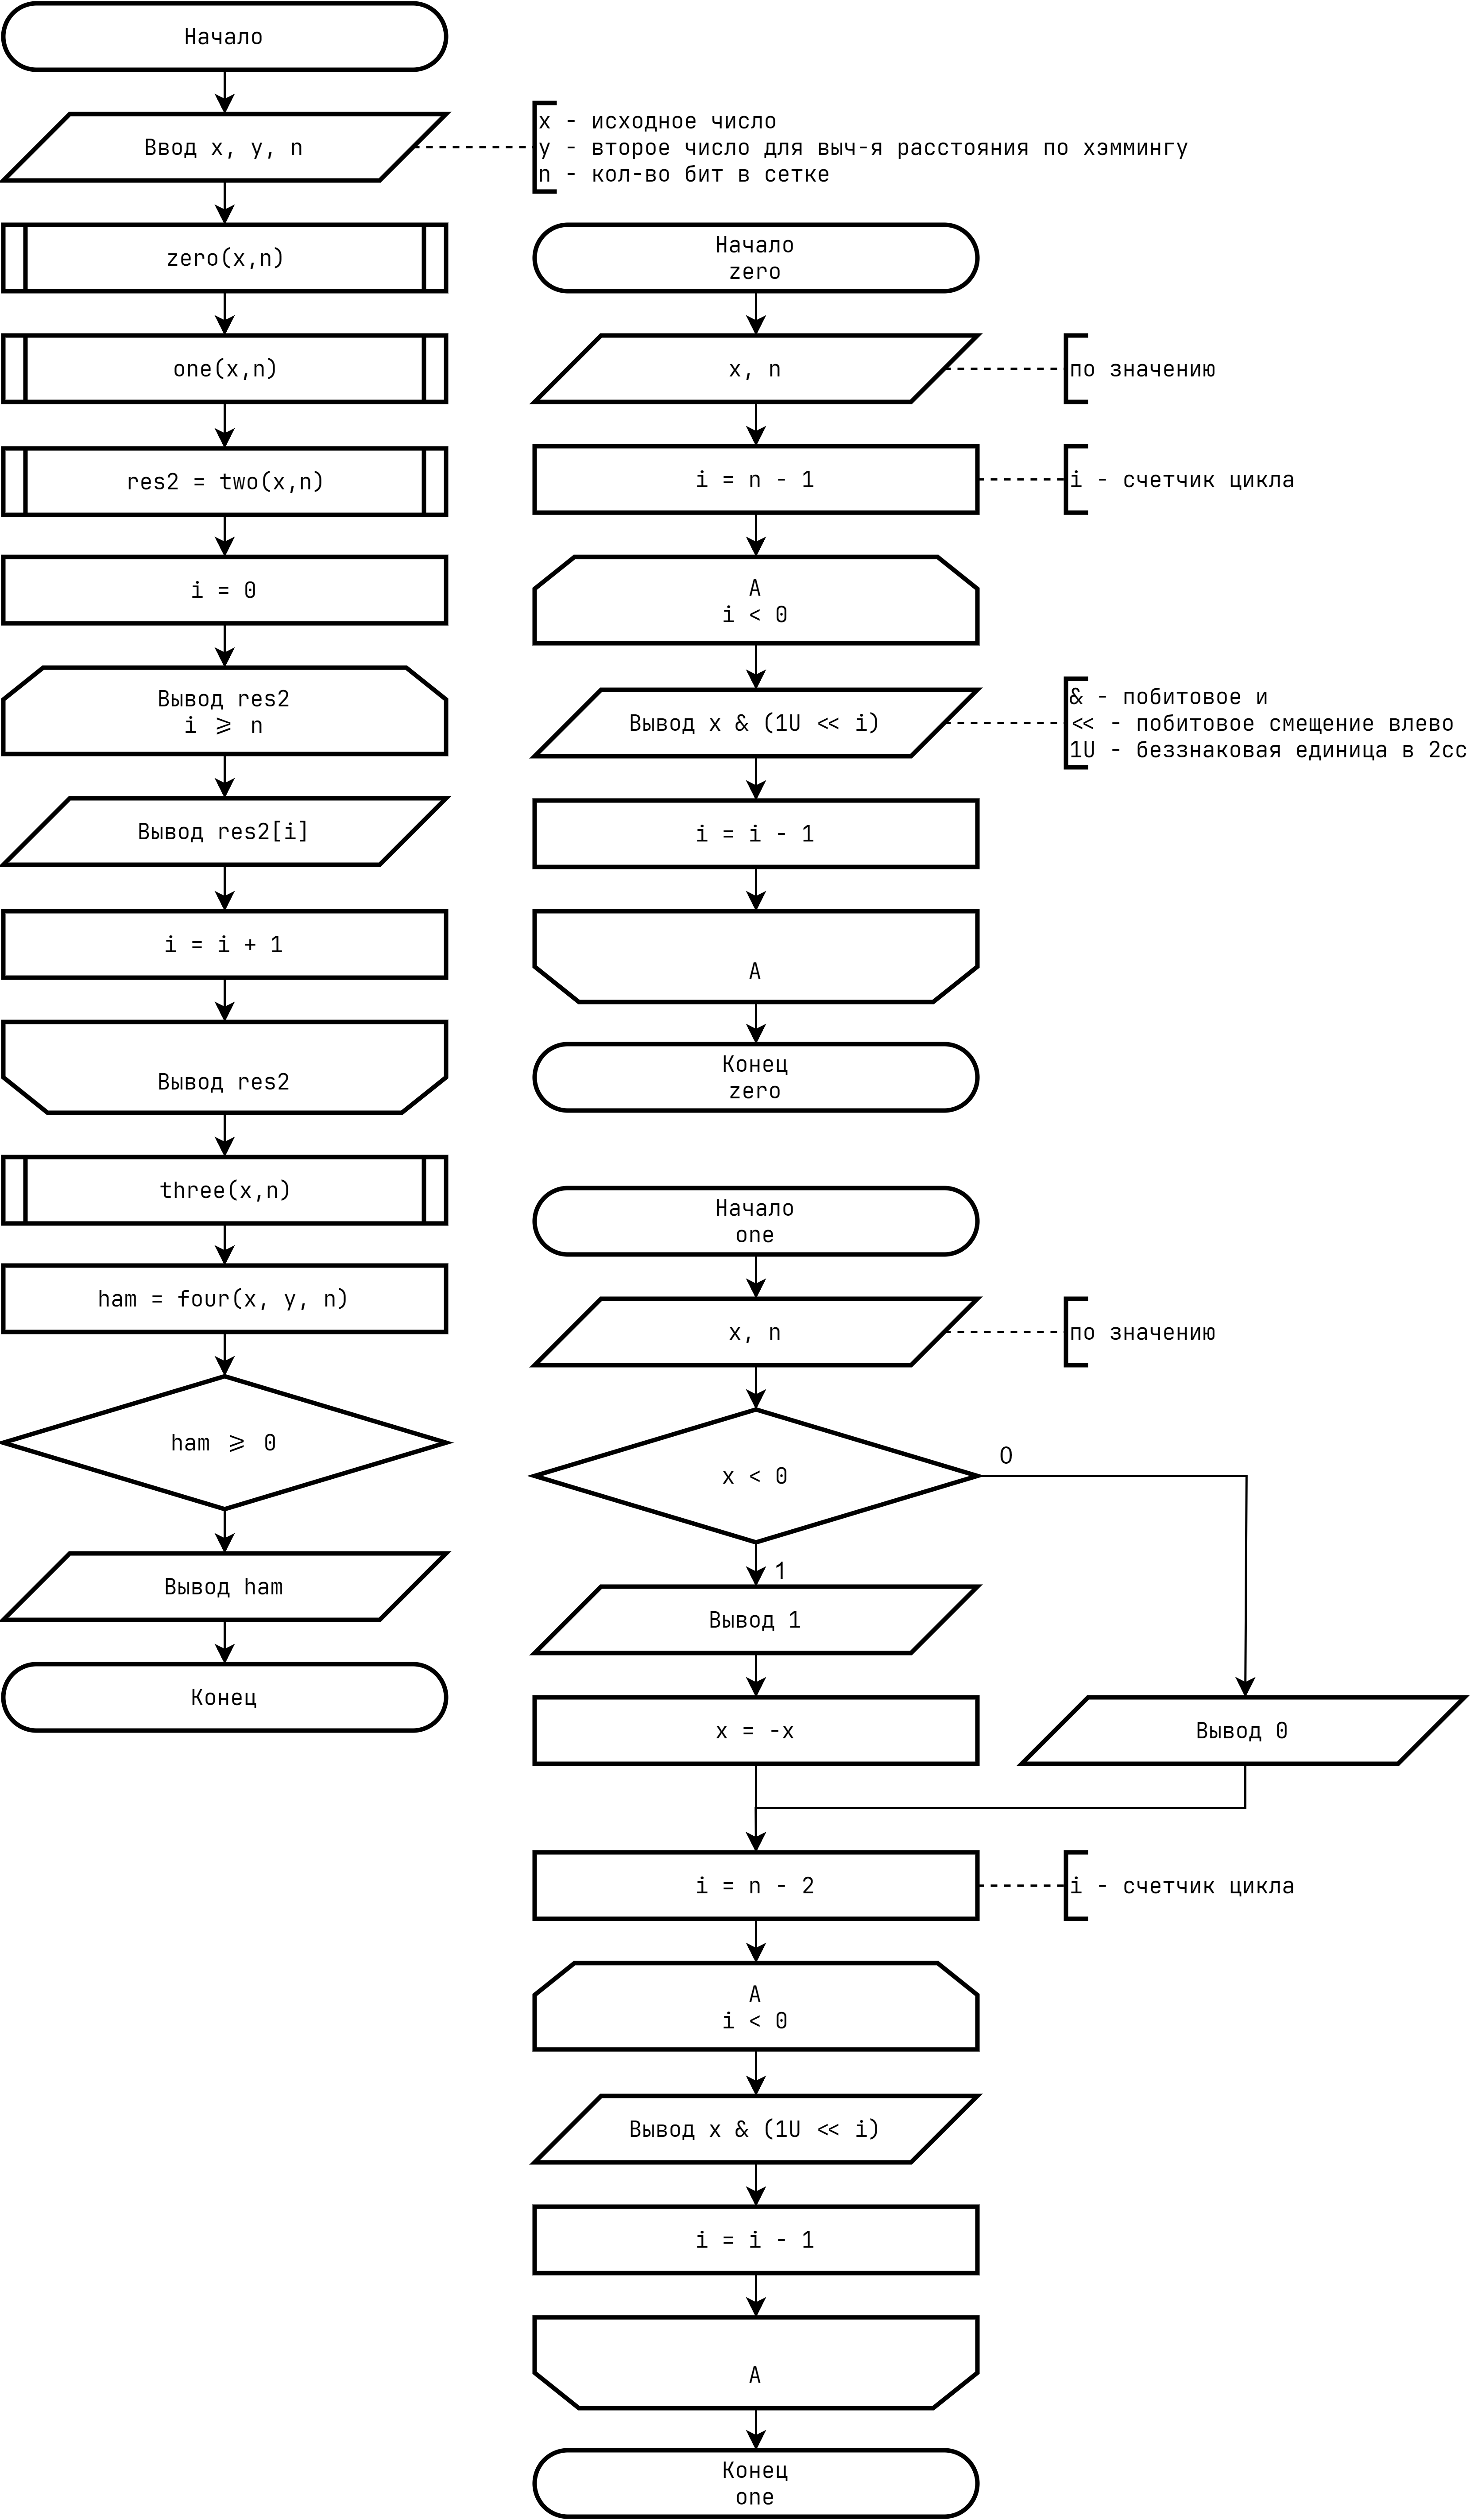
\includegraphics[width=0.8\textwidth]{pics/flowchart_p1.png}
	\caption*{Рисунок 1.1 - Схема алгоритма.}
\end{figure}

\begin{figure}[!ht]
	\centering
	%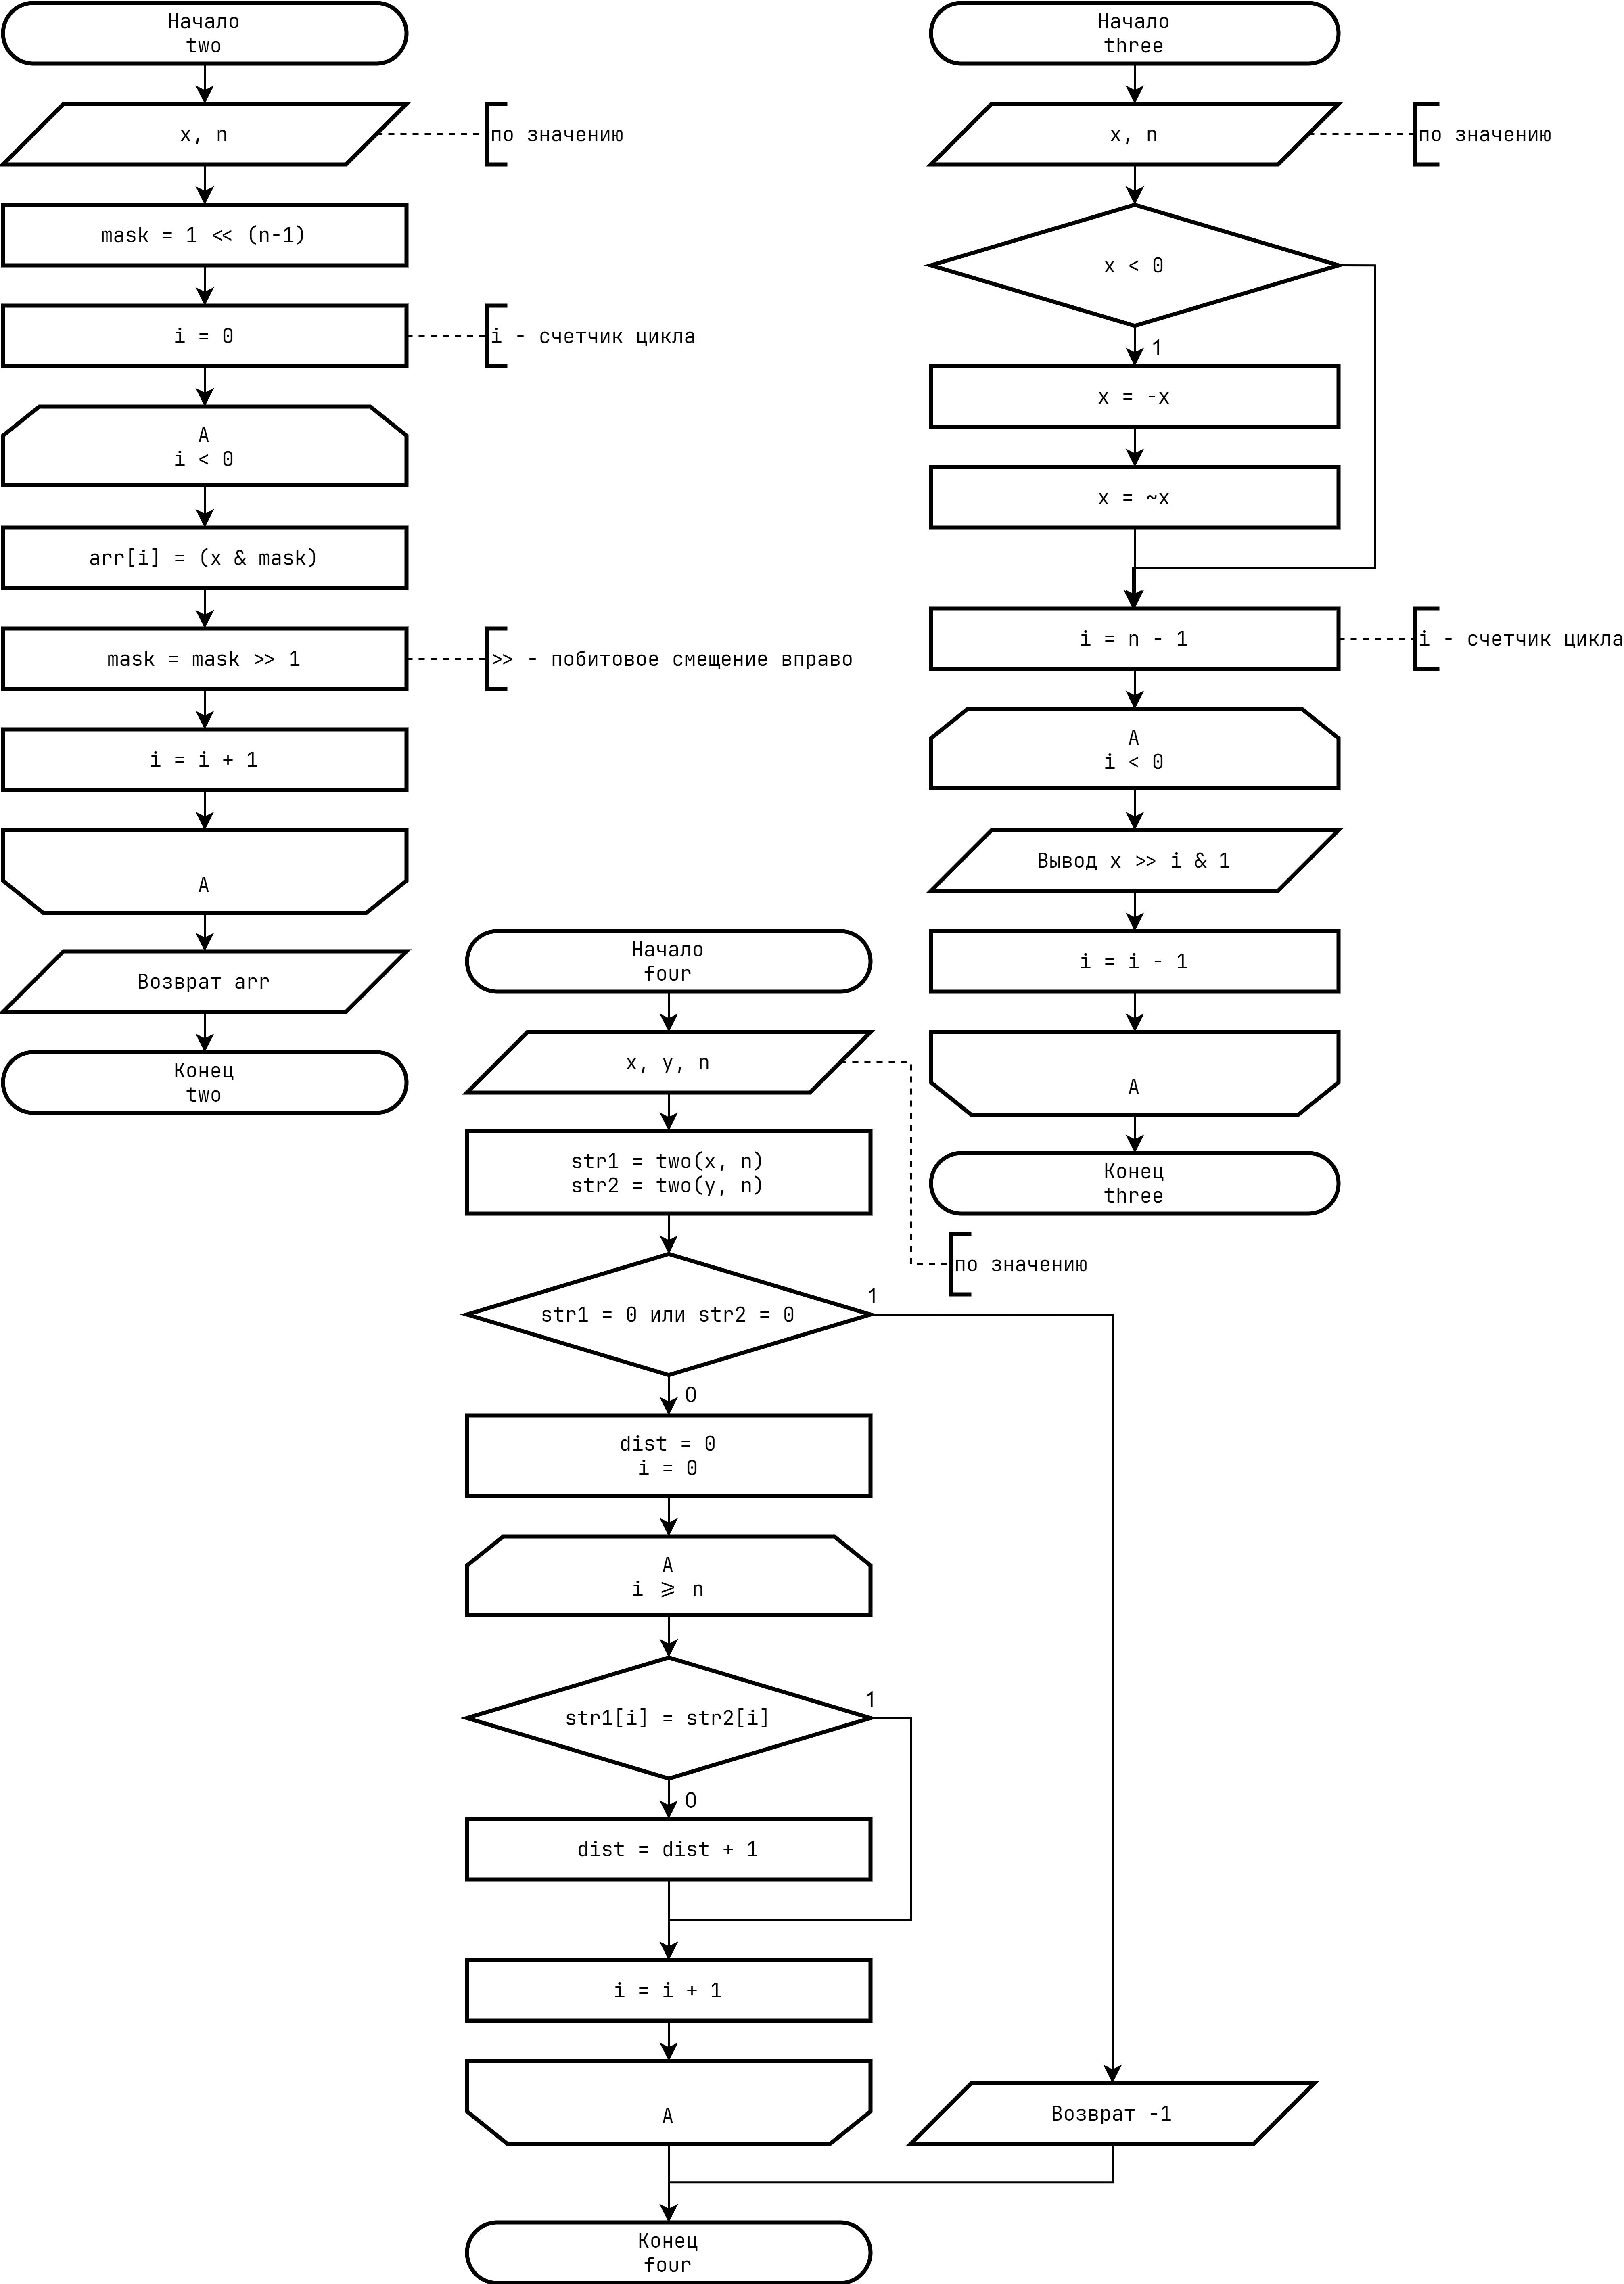
\includegraphics[height=0.9\textheight]{pics/flowchart_p2.png}
	\caption*{Рисунок 1.2 - Схема алгоритма.}
\end{figure}

\begin{figure}[!ht]
	\centering
	%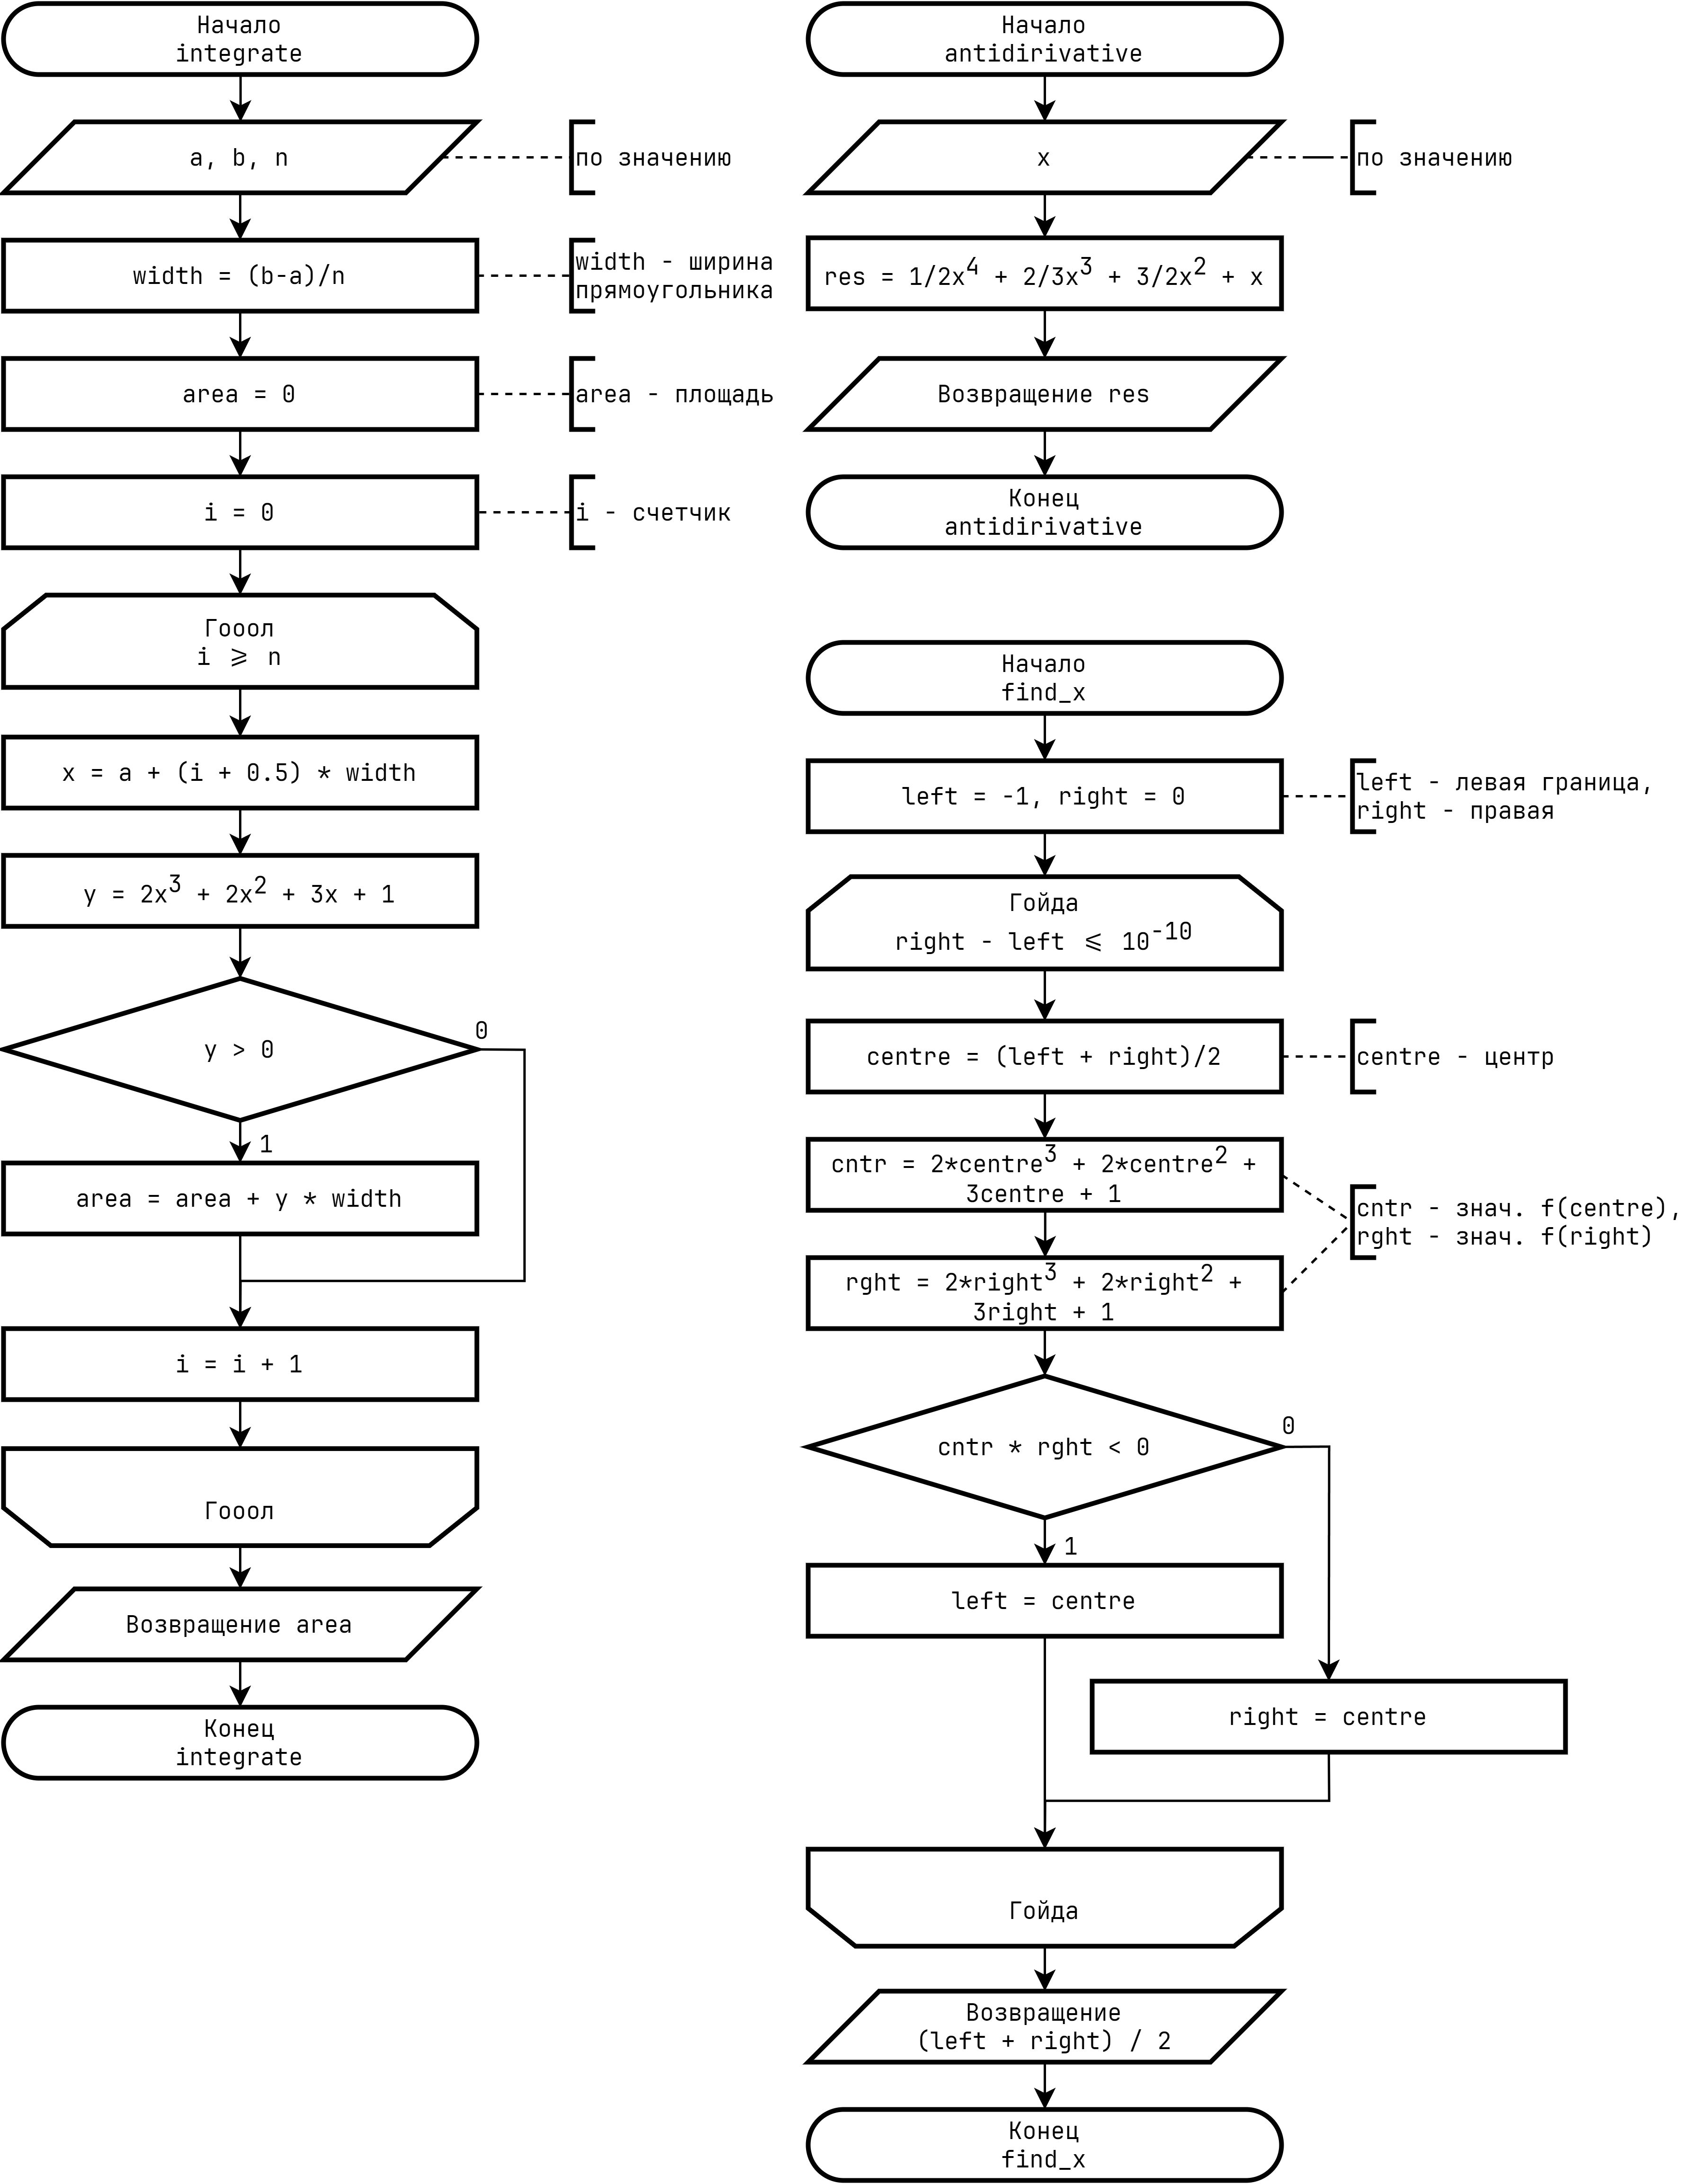
\includegraphics[height=0.9\textheight]{pics/flowchart_p3.png}
	\caption*{Рисунок 1.3 - Схема алгоритма.}
\end{figure}

\section*{Вывод}

В ходе выполнения работы изучены основы работы с двусвязным списком, реализованы операции добавления и удаления элементов, а также организован интерактивный пользовательский интерфейс для управления списком.

\newpage
\section*{Приложение А1. Исходный код}

\VerbatimInput[fontsize=\small]{code/main.c}

\end{document}
